% !TeX spellcheck = en_US
% !TeX encoding = utf8
% !TeX program = xelatex
% !BIB program = bibtex

\documentclass[notes]{beamer}
% \documentclass[draft]{beamer}	
\usetheme{Singapore}
% \usetheme{Hannover}
%\usepackage{pgfpages}
%\setbeameroption{show notes on second screen}

\usepackage[british]{babel}
\usepackage{graphicx,hyperref,url}
% \usepackage{ru}
\usepackage{mmstyles}
% \usepackage{hanging}
\usepackage{listings}
\usefonttheme[onlymath]{serif}
\usepackage{fontspec}
\usepackage{xeCJK}
% \pgfdeclareimage[width=\paperwidth,height=\paperheight]{bg}{background}
% \setbeamertemplate{background}{\pgfuseimage{bg}}
%% columns
\newcommand{\begincols}[1]{\begin{columns}{#1}}
\newcommand{\stopcols}{\end{columns}}
% \usepackage[backend=biber]{biblatex}
% \bibliography{./ref.bib}
%\addbibresource{ref.bib}
\usepackage{indentfirst}
\usepackage{longtable}
\usepackage{float}
%\usepackage{picins}
\usepackage{rotating}
\usepackage{subfigure}
\usepackage{tabu}
\usepackage{amsmath}
\usepackage{amssymb}
\usepackage{setspace}
\usepackage{amsfonts}
\usepackage{appendix}
\usepackage{listings}
\usepackage{xcolor}
\usepackage{geometry}
% \setCJKfamilyfont{cjkhwxk}{SimSun}
% \newcommand*{\cjkhwxk}{\CJKfamily{cjkhwxk}}
%\newfontfamily{\consolas}{Consolas}
%\newfontfamily{\monaco}{Monaco}
%\setmonofont[Mapping={}]{Consolas}	%英文引号之类的正常显示,相当于设置英文字体
%\setsansfont{Consolas} %设置英文字体 Monaco, Consolas,  Fantasque Sans Mono
% \setmainfont{Times New Roman}
% \newfontfamily{\consolas}{Times New Roman}
% \newfontfamily{\monaco}{Arial}
% \setCJKmainfont{Times New Roman}
%\setmainfont{MONACO.TTF}
%\setsansfont{MONACO.TTF}
\newcommand{\verylarge}{\fontsize{60pt}{\baselineskip}\selectfont}  
\newcommand{\chuhao}{\fontsize{44.9pt}{\baselineskip}\selectfont}  
\newcommand{\xiaochu}{\fontsize{38.5pt}{\baselineskip}\selectfont}  
\newcommand{\yihao}{\fontsize{27.8pt}{\baselineskip}\selectfont}  
\newcommand{\xiaoyi}{\fontsize{25.7pt}{\baselineskip}\selectfont}  
\newcommand{\erhao}{\fontsize{23.5pt}{\baselineskip}\selectfont}  
\newcommand{\xiaoerhao}{\fontsize{19.3pt}{\baselineskip}\selectfont} 
\newcommand{\sihao}{\fontsize{14pt}{\baselineskip}\selectfont}      % 字号设置  
\newcommand{\xiaosihao}{\fontsize{12pt}{\baselineskip}\selectfont}  % 字号设置  
\newcommand{\wuhao}{\fontsize{10.5pt}{\baselineskip}\selectfont}    % 字号设置  
\newcommand{\xiaowuhao}{\fontsize{9pt}{\baselineskip}\selectfont}   % 字号设置  
\newcommand{\liuhao}{\fontsize{7.875pt}{\baselineskip}\selectfont}  % 字号设置  
\newcommand{\qihao}{\fontsize{5.25pt}{\baselineskip}\selectfont}    % 字号设置 

\graphicspath{{./fig/}}

% \setbeamertemplate{footnote}{%
%   \hangpara{2em}{1}%
%   \makebox[2em][l]{\insertfootnotemark}\footnotesize\insertfootnotetext\par%
% }

\definecolor{cred}{rgb}{0.6,0,0}
\definecolor{cgreen}{rgb}{0.25,0.5,0.35}
\definecolor{cpurple}{rgb}{0.5,0,0.35}
\definecolor{cdocblue}{rgb}{0.25,0.35,0.75}
\definecolor{cdark}{rgb}{0.95,1.0,1.0}
\lstset{
	language=R,
	numbers=left,
	numberstyle=\tiny\color{black},
	keywordstyle=\color{cpurple}\consolas,
	commentstyle=\color{cgreen}\consolas,
	stringstyle=\color{cred}\consolas,
	frame=single,
	escapeinside=``,
	xleftmargin=1em,
	xrightmargin=1em, 
	backgroundcolor=\color{cdark},
	aboveskip=1em,
	breaklines=true,
	tabsize=3
} 

\providecommand{\tightlist}{%
  \setlength{\itemsep}{0pt}\setlength{\parskip}{0pt}}

  
% The title of the presentation:
%  - first a short version which is visible at the bottom of each slide;
%  - second the full title shown on the title slide;
\title[Opt for ML]{Multilayer Perceptrons (MLPs)}

% Optional: a subtitle to be dispalyed on the title slide
% \subtitle{Optimization for Machine Learning}

% The author(s) of the presentation:
%  - again first a short version to be displayed at the bottom;
%  - next the full list of authors, which may include contact information;
\author[YingmingLi]{Yingming Li \\ yingming@zju.edu.cn}
% The institute:
%  - to start the name of the university as displayed on the top of each slide
%    this can be adjusted such that you can also create a Dutch version
%  - next the institute information as displayed on the title slide

\institute[DSERC, ZJU]{Data Science \& Engineering Research Center, ZJU}

% Add a date and possibly the name of the event to the slides
%  - again first a short version to be shown at the bottom of each slide
%  - second the full date and event name for the title slide
\date[\today]{\today}

\begin{document}

\AtBeginSection[]
{
	\begin{frame}
		\frametitle{Outline}
		\tableofcontents[currentsection]
	\end{frame}
}

% \AtBeginSubsection[2-]
% {
%    \begin{frame}
%        \frametitle{Outline}
%        \tableofcontents[currentsection]
%    \end{frame}
% }
\begin{frame}
	\titlepage
	\begin{center}
		Adapted from slides provided by Prof.  Michael Mandel.		
	\end{center}
\end{frame}
\section{}\label{section}

\begin{frame}{Motivation}

\begin{itemize}
\tightlist
\item
  Multilayer networks are more powerful than single layer nets

  \begin{itemize}
  \tightlist
  \item
    \eg, XOR problem
  \end{itemize}
\end{itemize}

\centering 

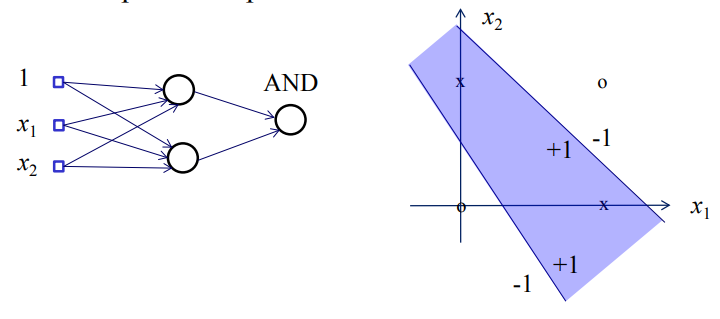
\includegraphics[width=0.70000\textwidth]{2018-03-10-11-05-54.png}\\

\end{frame}

\begin{frame}{Power of nonlinearity}

\begin{itemize}
\tightlist
\item
  For linear neurons, a multilayer net is equivalent to a single-layer
  net. This is not the case for nonlinear neurons

  \begin{itemize}
  \tightlist
  \item
    Why?
  \end{itemize}
\end{itemize}

\end{frame}

\begin{frame}{MLP architecture}

\centering 

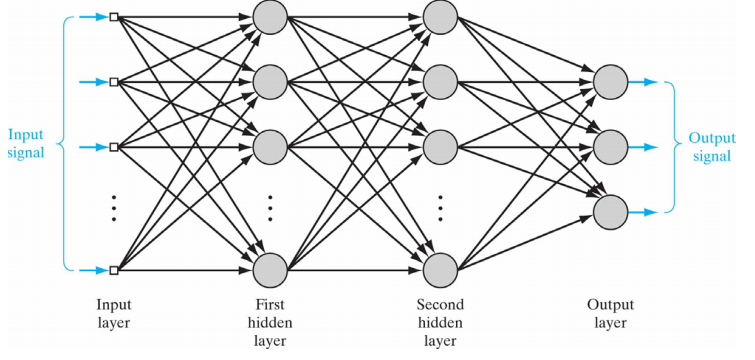
\includegraphics[width=0.80000\textwidth]{2018-03-10-11-08-20.png}\\

\end{frame}

\begin{frame}{Multi-layer perceptron}

\begin{itemize}
\tightlist
\item
  Think of an MLP as a complicated, non-linear function of its input
  parametrized by \(\vw\): \[\vy=F(\vx;\vw)\]
\item
  Note that ``Multi-layer perceptron'' is a bit of a misnomer because
  they use a continuous activation function
\end{itemize}

\end{frame}

\begin{frame}{MLP Training}

\begin{itemize}
\tightlist
\item
  Given a set of training data \(\{\vx_p,\vd_p\}\) can we adjust \(\vw\)
  so that the network is optimal
\item
  Optimal \wrt what criterion

  \begin{itemize}
  \tightlist
  \item
    Must define error criterion between \(\vy _\vp = F(\vx_\vp ; \vw)\)
    and \(\vd_p\)
  \item
    We will use the mean square error for now, but others are possible
    (and often preferable)
  \end{itemize}
\item
  Goal find \(\vw\) that minimizes
  \[  \bar{E}(\vw) = \sum_p E_p(\vw) = \sum_p \frac{1}{2} \|\vd_p - F(\vx_p ;\vw)\|^2\]
\end{itemize}

\end{frame}

\begin{frame}{Backpropagation}

Backpropagation will be continued on Thursday, March 18.

\end{frame}
\begin{frame}
	\chuhao Thank you! %\fontspec{LHANDW.TTF}
\end{frame}
\end{document}
